\section{Implementierung}
\subsection{Screenshot}
\begin{figure}[!htbp]
 \centering
 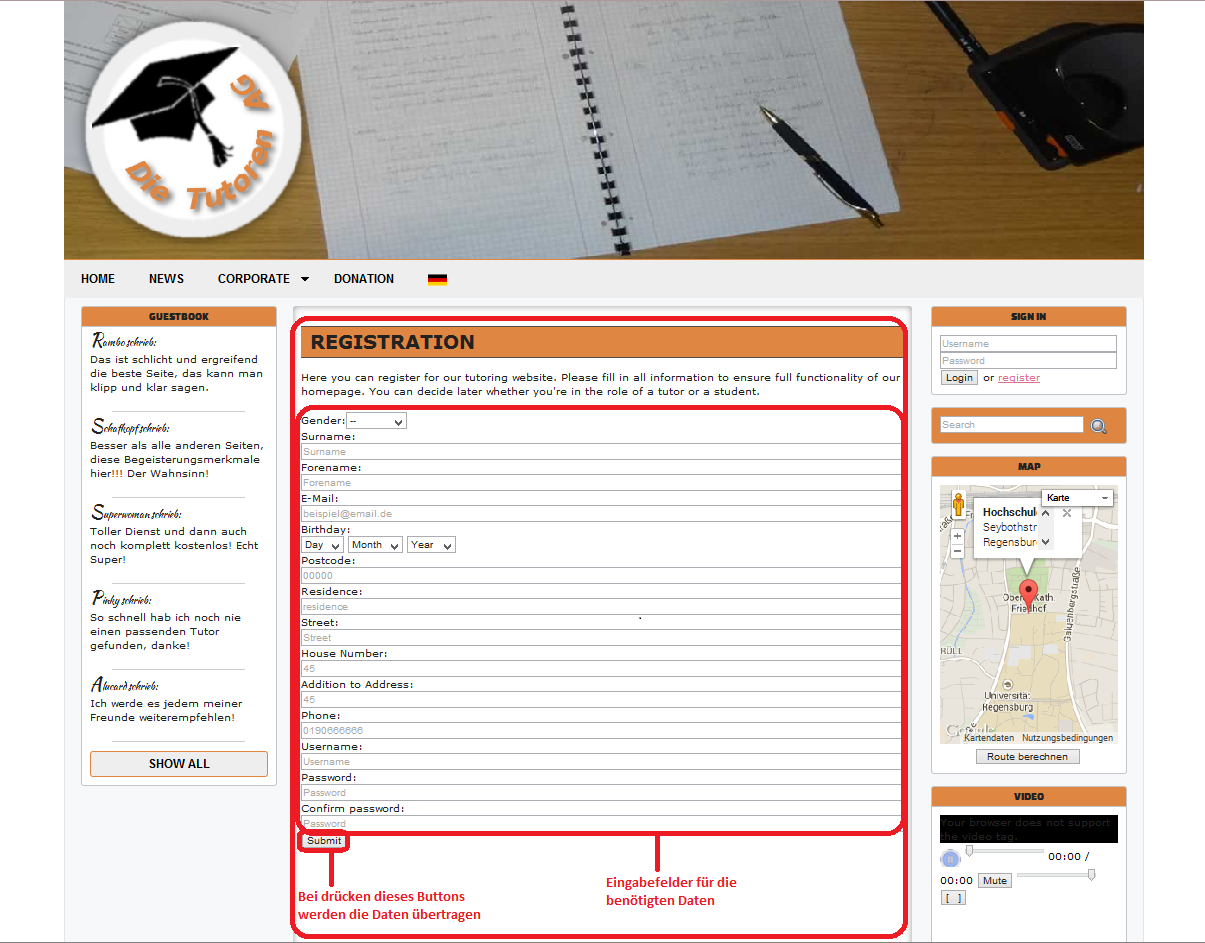
\includegraphics[scale=0.4]{./Screenshot/Register}
 \caption{Register}
 \label{fig:RegisterEn}
\end{figure}

\subsection{Code}
\defverbatim[colored]
  \makeset{
    \phpcode

      \begin{lstlisting}[name=registration.html]
	<select name="tag" id="tag" style="width:50"><option value="-1">Day</option>
	<?php
    $i = 0;
    while ( $i++ < 31)
    echo '<option value="'.$i.'">'.$i.'</option>';?></select>
	<select name="monat" id="monat">
	<option value="-1">Month</option>
	<?php
	$i = 0;
	while ( $i++ < 12)
	echo '<option value="'.$i.'">'.$i.'</option>';?>
	</select>
	<select name="jahr" id="jahr">
	<option value="-1">Year</option>
	<?php
    $i = date("Y");
    while ( $i-- > 1900)
    echo '<option value="'.$i.'">'.$i.'</option>';?>
	</select></div>
      \end{lstlisting}
}

\begin{frame}
  \frametitle{Selectbox für Datum}
  \makeset
\end{frame}
\defverbatim[colored]
  \makeset{
    \jscode

      \begin{lstlisting}[name=registration.js]
	$(document).ready(function()
	{
    $.post("/scripts/GetLang.php", function(lang) {
        if (lang.length > 2) {  /*Wenn Englisch wird dieser Teil genutzt*/
            

      \end{lstlisting}
}

\begin{frame}
  \frametitle{Sprache der Session}
  \makeset
\end{frame}

\defverbatim[colored]
  \makeset{
    \jscode

      \begin{lstlisting}[name=registration.js]
				$.validator.addMethod('phone', function(value) {
                var numbers = value.split(/\d/).length - 1;
                return (2 <= numbers && numbers <= 15 && value.match(/^(\+){0,1}(\d|\s|\(|\)){2,15}$/));
            }, 'Please enter a valid phone number');
      \end{lstlisting}
  }

\begin{frame}
  \frametitle{Eigene JQuery-Validate-Methode}
  \makeset
\end{frame}

\defverbatim[colored]
  \makeset{
    \jscode

      \begin{lstlisting}[name=registration.js]
            $("#registerform").validate({
                errorPlacement: function(error, element) {
                    if (element.attr("name") === "jahr") {
                        element.prev('label').replaceWith(error);
                    }
                    else if (element.attr("name") === "monat") {
                        element.prev('label').replaceWith(error);
                    } else {
                        error.insertBefore(element);
                    }
                },
      \end{lstlisting}
  }

\begin{frame}
  \frametitle{Fehlermeldungspositionen verändern}
  \makeset
\end{frame}

\defverbatim[colored]
  \makeset{
    \jscode

      \begin{lstlisting}[name=registration.js]
                rules: {
                    plz: {
                        number: true,
                        minlength: 5,
                        maxlength: 5
                    },
                    geschlecht: {
                        min: 0                     },
                    tag: {
                        min: 1                     },
                    jahr: {
                        min:                     },
                    monat: {
                        min: 1                    },
                    telefon: {
                        phone: true                    },
                    hausnummer: {
                        number: true                    }
                },

      \end{lstlisting}
  }

\begin{frame}
  \frametitle{Validation Regeln zuweisen}
  \makeset
\end{frame}

\defverbatim[colored]
  \makeset{
    \jscode

      \begin{lstlisting}[name=registration.js]
               messages: {/*Spezielle Texte fuer bestimmte Fehleingaben*/
                    plz: {
                        number: "A Postcode can only contain numbers",
                        minlength: jQuery.validator.format("A Postcode has only 5 digits."),
                        maxlength: jQuery.validator.format("A Postcode has only 5 digits.")
                    },
                    tag: {
                        min: jQuery.validator.format("Please enter a valid Date.")
                    },
                    monat: {
                        min: jQuery.validator.format("Please enter a valid Date.")
                    },
                    telefon: {
                        phoneUS: "Please enter a valid phone number"
                    },
                    jahr: {
                        min: jQuery.validator.format("Please enter a valid Date.")
                    },
                    geschlecht: {
                        min: jQuery.validator.format("Please select a gender.")
                    }
                },
      \end{lstlisting}
  }

\begin{frame}
  \frametitle{Fehlermeldungstexte 1}
  \makeset
\end{frame}

\defverbatim[colored]
  \makeset{
    \jscode

      \begin{lstlisting}[name=registration.js]
               jQuery.extend(jQuery.validator.messages, {/*Veraenderungen an den Standartfehlermeldungen Englisch*/
                required: "This field is required by us!.",
                remote: "Please fix this field.",
                email: "Please enter a valid email address.",
                url: "Please enter a valid URL.",
                date: "Please enter a valid date.",
                dateISO: "Please enter a valid date (ISO).",
                number: "Please enter a valid number.",
                digits: "Please enter only digits.",
                creditcard: "Please enter a valid credit card number.",
                equalTo: "Please enter the same value again.",
                accept: "Please enter a value with a valid extension.",
                maxlength: jQuery.validator.format("Please enter no more than {0} characters."),
                minlength: jQuery.validator.format("Please enter at least {0} characters."),
                rangelength: jQuery.validator.format("Please enter a value between {0} and {1} characters long."),
                range: jQuery.validator.format("Please enter a value between {0} and {1}."),
                max: jQuery.validator.format("Please enter a value less than or equal to {0}."),
                min: jQuery.validator.format("Please enter a value greater than or equal to {0}.")
            }
      \end{lstlisting}
  }

\begin{frame}
  \frametitle{Fehlermeldungstexte 2}
  \makeset
\end{frame}

\defverbatim[colored]
  \makeset{
    \jscode
      \begin{lstlisting}[name=registration.js]
					invalidHandler: function(event, validator) {/*Ausgabe der Fehler*/
                    var errors = validator.numberOfInvalids();/*Anzahl der Fehler*/
                    if (errors) {
                        var message = (errors === 1) ? 'You missed 1 field. It has been highlighted' : 'You missed ' + 								errors + ' fields. They have been highlighted';
                        $("div.error span").html(message);
                        $("div.error").show();
                        alert(message.toString());
                    } else {
                        $("div.error").hide();
                    }
                },
      \end{lstlisting}
  }

\begin{frame}
  \frametitle{Ausgabe}
  \makeset
\end{frame}
\defverbatim[colored]
  \makeset{
    \jscode
      \begin{lstlisting}[name=registration.js]
					submitHandler: function(form) {
                    $.post("/scripts/CreateUser.php", $("#registerform").serialize(), /*Daten an PHP Script uebergeben*/
                            function(msg) {
                                /* msg ist leer, außer fehlgeschlag, dann wird der Fehler ausgegeben */
                                if (msg.length > 2) {
                                    alert(msg.toString());
                                }
                                /* Nur bei erfolgreicher Registrierung wird die Seite neu geladen */
                                if (msg.length < 5) {
                                    alert("The registration was successful, please wait till you get unlocked.");
                                    location.replace('index.php');
                                }
                            });
                }
      \end{lstlisting}
  }

\begin{frame}
  \frametitle{Übertragung}
  \makeset
\end{frame}

\subsection{Demonstration}
\begin{frame} %%Eine Folie
  \frametitle{Demonstration} %%Folientitel

% Fettgedruckt
  \center
  \textbf{Es folgt eine Demonstration ...}
\end{frame}

\subsection{Ende}
\begin{frame}
  \frametitle{Ende}
  \center
 \textbf{\highlighton{Vielen Dank für Ihre Aufmerksamkeit}}
\end{frame}